\section{\maestro\ Basics}

\maestro\ models problems that are in tight hydrostatic equilibrium.
The fluid state is decomposed into a 1D radial base state that
describes the hydrostatic structure of the star or atmosphere, and a
2- or 3D Cartesian full state, that captures the departures from
hydrostatic equilibrium.  Two basic geometries are allowed.  A {\em
  plane-parallel} geometry assumes that the domain is thin compared to
the radius of curvature of the star, and therefore the 1D base state
is perfectly aligned with the Cartesian state.  A {\em spherical}
geometry is for modeling an entire star.  Here, the 1D base state is
not aligned with the Cartesian state.  Figure~\ref{fig:base_state}
shows these geometries.

\begin{figure}[tb]
\centering
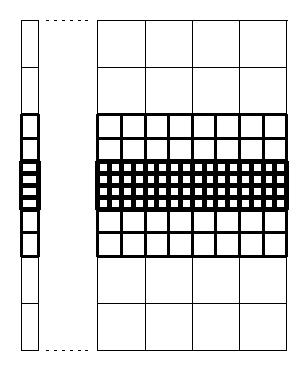
\includegraphics[height=2.0in]{\archfigpath/base_grid} \hspace{0.5in}
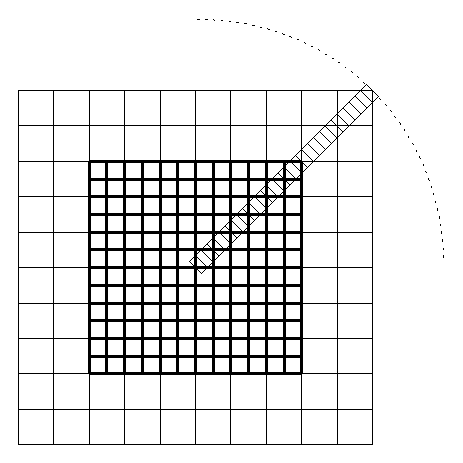
\includegraphics[height=2.0in]{\archfigpath/base_spherical}
\caption[\maestro\ geometries]{\label{fig:base_state} \maestro\ geometries, showing both the
  1D base state and the full Cartesian state.  (Left) For multi-level
  problems in planar geometry, we force a direct alignment between the
  radial array cell centers and the Cartesian grid cell centers by
  allowing the radial base state spacing to change with space and
  time.  (Right) For multi-level problems in spherical geometry, since
  there is no direct alignment between the radial array cell centers
  and the Cartesian grid cell centers, we choose to fix the radial
  base state spacing across levels. Figure taken
  from~\cite{multilevel}.}
\end{figure}


\maestro\ can use adaptive mesh refinement to focus resolution on
complex regions of flow.  For Cartesian/plane-parallel geometries, all
cells at the same height must be at the same level of refinement.
This restriction is to allow for the base state to directly align with
the Cartesian state everywhere.  For spherical geometries, there is no
such restriction (again, see Figure~\ref{fig:base_state}).
The \maestro\ grids are managed by the \boxlib\ library, which is
distributed separately.



\section{\maestro\ Directory Structure}

\begin{figure}[t]
\centering
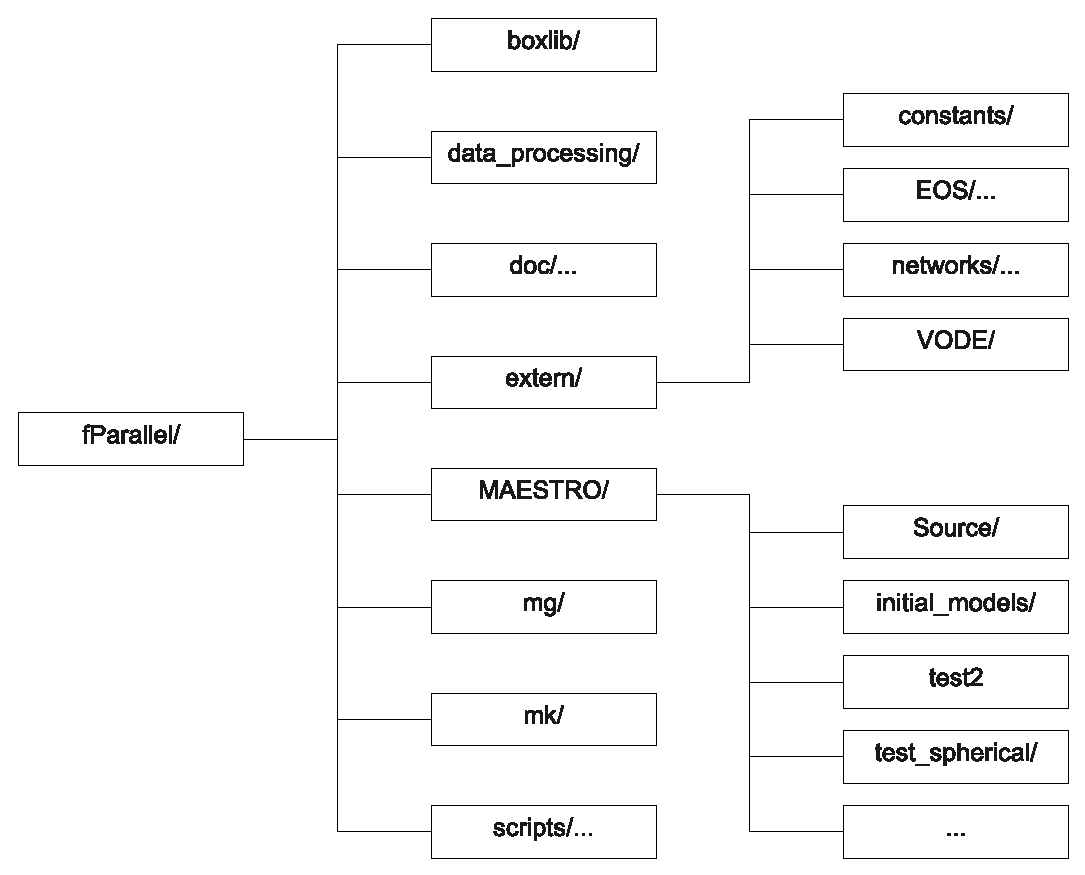
\includegraphics[scale=0.65]{\archfigpath/maestro_directory2}
\caption[\maestro\ directory structure]
{The basic \maestro\ directory structure.}
\end{figure}


Building \maestro\ requires both the \maestro-specific source
files (distributed in the {\tt MAESTRO/} directory), and the
\boxlib\ library (distributed in the {\tt BoxLib/} directory.
\boxlib\ provides both a C++ and a Fortran framework.  \maestro\
only uses the Fortran framework.

Problems piece together various \maestro\ directories, choosing a
reaction network, equation of state, and conductivity routine to build
an executable.  Briefly, the \maestro\ sub-directories are:
\begin{itemize}
\item {\tt data\_processing/}

  Simple Fortran-based analysis routines (e.g.\ extract a line from a
  multidimensional dataset) that operate on BoxLib datasets.

\item {\tt extern/}

  External modules, like ODE integrators, equations of state, reaction
  networks

  Important sub-directories include:
 
  \begin{itemize}
  \item {\tt conductivity/}

    Various routines for computing the thermal conductivity used in the
    thermal diffusion part of the algorithm.

  \item {\tt constants/}

    A simple module to define physical constants

  \item {\tt EOS/}

    A collection of various EOSes for use with the code.  The two
    important ones for \maestro\ are {\tt helmeos/} and {\tt
    gamma\_law\_general/}.

  \item {\tt model\_parser/}

    A simple Fortran module for reading in 1D initial model files.
    This is used by the initialization routines to get the initial
    model data.

  \item {\tt networks/}

    Various reaction networks for \maestro\ problems.  In addition to
    providing a routine to evolve the nuclear species due to
    reactions, the networks also define the species that are advected
    by the code.

  \item {\tt VODE/}

    An integration package for ODEs.  At the moment, this is used for
    integrating various reaction networks.
 
  \end{itemize}

\item {\tt MAESTRO/}

  The main \maestro\ algorithm directory.  The individual problem
  directories lie under here, and all of the main \maestro\ source
  lives in the {\tt Source/} sub-directory.

  Important directories under {\tt MAESTRO/} include:

  \begin{itemize}

  \item {\tt docs/}

    Documentation describing the basic algorithm (including this
    document).

  \item {\tt initial\_models}

    Several sub-directories containing routines to generate 1D initial
    conditions in hydrostatic equilibrium for mapping onto the
    \maestro\ grid.  See \S~\ref{sec:initial_models} for details.

  \item {\tt Source}

    The main \maestro\ source.  Here you will find the driver routine,
    the advection routines, etc.  All \maestro\ problems will compile
    this source.

  \item problem directories: {\tt test2}, {\tt test\_spherical},
    $\ldots$

    Each problem in \maestro\ gets it own sub-directory.  The {\tt
      GNUmakefile} in the problem directory includes the instructions
    on how to build the executable, including what modules in {\tt
      extern} are used.

    Any file that you place in a sub-directory here takes precedence
    over a file of the same name in {\tt MAESTRO/}.  This allows
    problems to have custom versions of the main \maestro\ routines
    (e.g.\ initial conditions via {\tt initdata.f90}.  See
    \S~\ref{sec:makefile} for details on the build system).

  \end{itemize}

\end{itemize}


\begin{figure}[t]
\centering
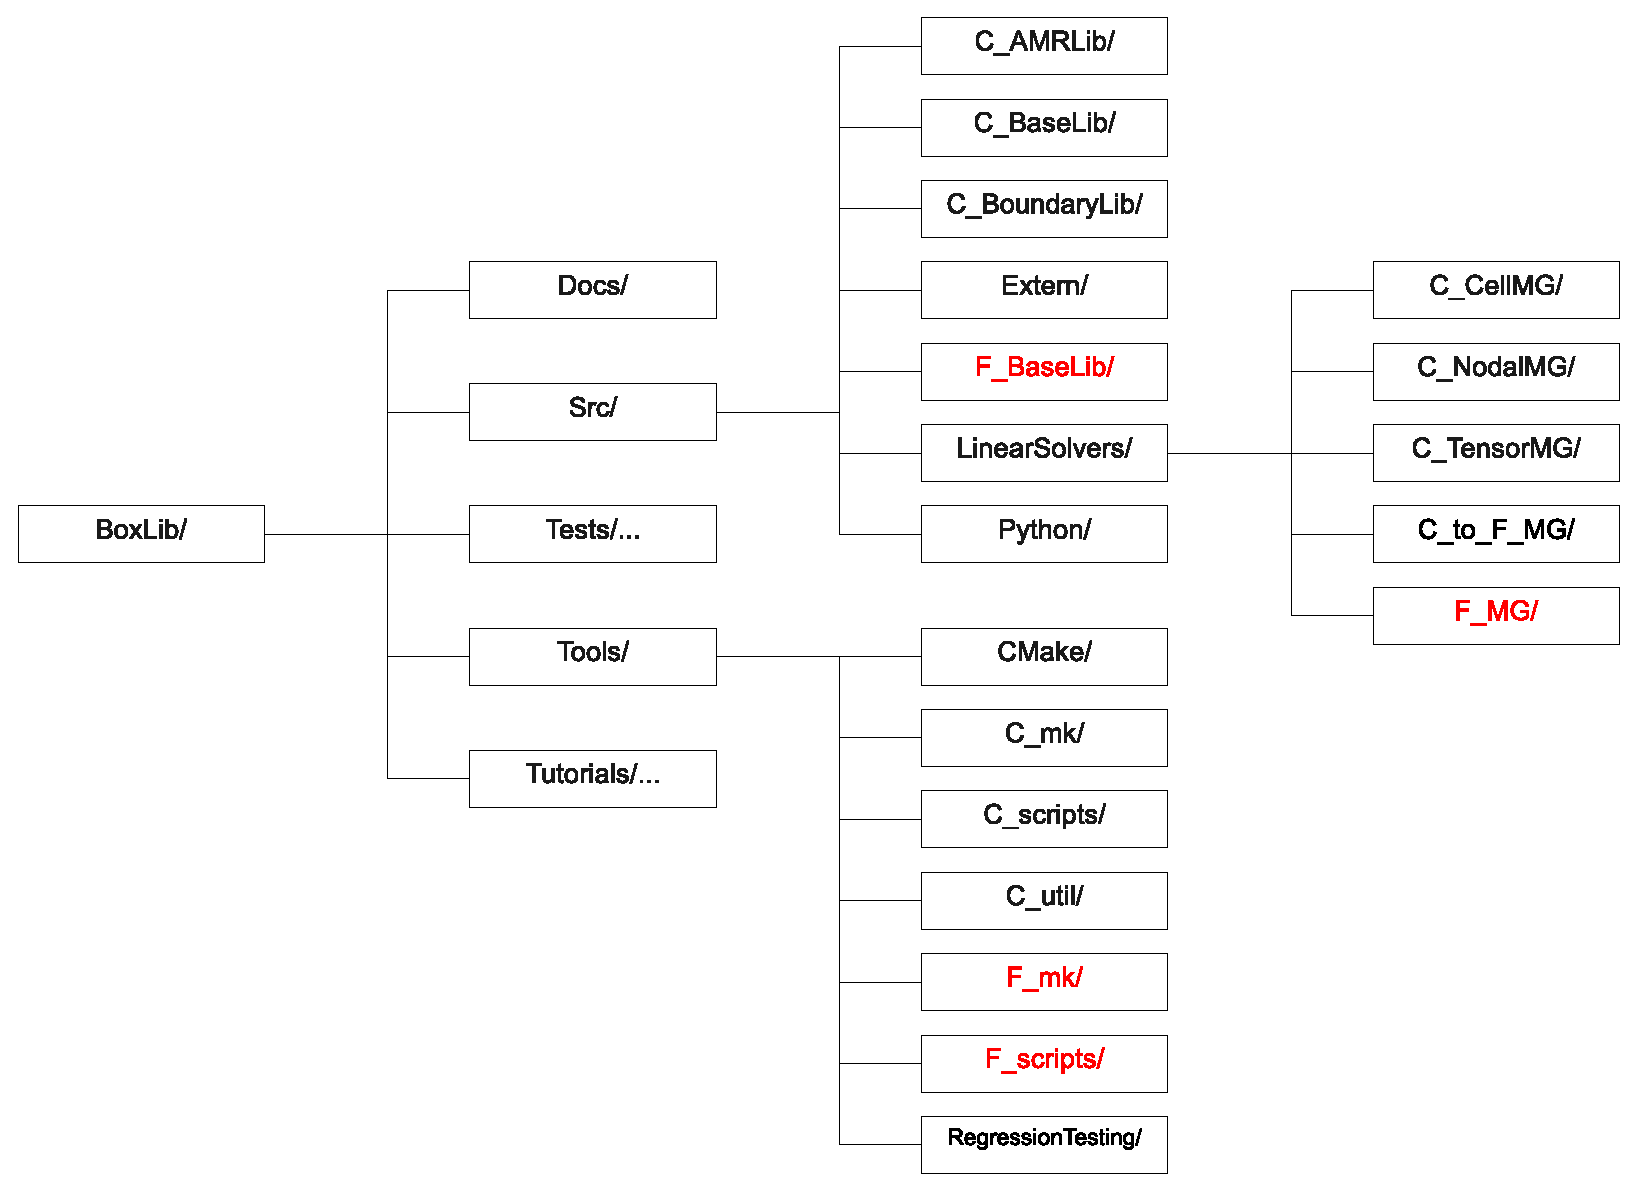
\includegraphics[scale=0.65]{\archfigpath/boxlib_directory2}
\caption[\boxlib\ directory structure]
{The basic \boxlib\ directory structure.  The directories used
by \maestro\ are indicated in red.}
\end{figure}

The \boxlib\ directories that \maestro\ uses are:
\begin{itemize}
\item {Src/}

  The main \boxlib\ source directory.  In \maestro, we only use the
  Fortran source files.  The core directories are:

  \begin{itemize}

  \item {\tt F\_BaseLib/} 

    The Fortran \boxlib\ files.  This is a library for describing
    meshes consisting of a union of boxes.  The \boxlib\ modules
    define the basic datatypes used in \maestro.  \boxlib\ also
    provides the routines that handle the parallelization and I/O.

  \item {\tt LinearSolvers/}

    The \boxlib\ linear solvers---these are used to solve elliptic
    problems in the \maestro\ algorithm.

    \begin{itemize}

    \item {\tt F\_MG}

      The Fortran multigrid solver, with support for both
      cell-centered and node-centered data.

    \end{itemize}

  \end{itemize}

\item {\tt Tools/}

  Various tools used for building \boxlib\ applications.  Here we use:

  \begin{itemize}

  \item {F\_mk/}

    The generic Makefiles that store the compilation flags for various
    platforms.  Platform/compiler-specific options are stored in the
    {\tt comps/} sub-directory.

  \item {\tt F\_scripts/}

    Some simple scripts that are useful for building, running,
    maintaining \maestro.

  \end{itemize}

\end{itemize}






\section{Unit Tests}

\label{sec:unit_tests}

In addition to the problems described above which use the full
capabilities of \maestro, there are a number of unit tests that
exercise only specific components of the \maestro\ solvers.  The
tests have their own drivers (a custom {\tt varden.f90}) that
initialize only the data needed for the specific test and call
specific \maestro\ routines directly.

\begin{itemize}
\item {\tt test\_advect} \\[-3mm]

  This test initializes a Gaussian density field (no other scalar
  quantities are used) and a uniform velocity field in any one of the
  coordinate directions.  The Gaussian profile is advected through
  the period domain exactly once and the error in the density profile
  (L2 norm) is computed.  The driver for this problem does this 
  for every dimension twice (once with a positive velocity and once
  with a negative velocity).  After all coordinate directions are 
  tested, the norms are compared to ensure that the error does
  not show any directional bias.


\item {\tt test\_average} \\[-3mm]

  This test initializes a 1D radial base state quantity with a
  Gaussian distribution, maps it into the 3D domain (assuming a
  spherical geometry) using the routines provided by the {\tt
    fill\_3d\_module} module, and then calls {\tt average} to put it
  back onto a 1D radial array.  This way we test the accuracy of our
  procedure to map between the 1D radial and 3D Cartesian states.
  The output from this test was described in detail in
  \cite{multilevel}.

\item {\tt test\_basestate} \\[-3mm]

  This test initializes the base state to contain a hydrostatic
  model and then evolves the state with heating to watch the 
  hydrostatic adjustment of the atmosphere.  In particular,
  the base state velocity, $w_0$, is computed in response to 
  the heating and this is used to advect the base state density
  and compute the new pressure, $p_0$.  An early version of 
  this routine was used for the plane-parallel expansion test
  in \cite{lowMach2}.  This version of the test was also shown
  for a spherical, self-gravitating star in \cite{multilevel}.

  
\item {\tt test\_diffusion}

  This test initializes a Gaussian temperature profile and calls
  the thermal diffusion routines in \maestro\ to evolve the state 
  considering only diffusion.  The driver estimates a timestep
  based on the explicit thermal diffusion timescale and loops
  over calls to the thermal diffusion solver.  A Gaussian remains
  Gaussian when diffusing, so an explicit error can be computed
  by comparing to the analytic solution.  This test is 
  described in \cite{xrb}.


\item {\tt test\_particles}

  This test exercises the particle advection routine.  A simple
  circular velocity field, with the magnitude increasing with radius
  from the center is initialized.  A number of particles are then
  initialized at various radii from the center and they are advected
  for one period.  The particle paths should be perfect circles, and
  the final particle position should overlap with the initial
  position.

  Particle data is stored separately from the fluid data.  Instead
  of being part of the plotfiles, the particle data is outputted
  each timestep into files named {\tt timestamp\_*}, where 
  the number indicates which processor did the writing.  These
  particle files can be processed and the particle data plotted
  using the python routines in {\tt data\_processing/python/}.

\end{itemize}


\section{Adding A New Problem}
\label{sec:adding_problems}

Different \maestro\ problems are defined in sub-directories under
{\tt MAESTRO/}.  To add a problem, start by creating a new
sub-directory---this is where you will compile your problem and
store all the problem-specific files.

The minimum requirement to
define a new problem would be a {\tt GNUmakefile} which describes how
to build the application and an input file which lists the runtime
parameters.  The problem-specific executable is built in the problem
directory by typing {\tt make}.  Source files are found automatically
by searching the directories listed in the {\tt GNUmakefile}.
Customized versions of any source files placed in the problem-directory
override those with the same name found elsewhere.  Any unique
source files (and not simply a custom version of a file found
elsewhere) needs to be listed in a file call {\tt GPackage.mak}
in the problem-directory.

\subsection{The {\tt GNUmakefile}}

\label{sec:makefile}

A basic {\tt GNUmakefile} begins with:
\begin{lstlisting}[language={[gnu]make},mathescape=false]
  NDEBUG := t
  MPI    :=
  OMP    :=
\end{lstlisting}
Here, {\tt NDEBUG} is true if we are building an optimized executable.
Otherwise, the debug version is built---this typically uses less
optimization and adds various runtime checks through compiler flags.
{\tt MPI} and {\tt OMP} are set to true if we want to use either MPI
or OpenMP for parallelization.  If {\tt MPI := t}, you will need to
have the MPI libraries installed, and their location may need to be 
specified in {\tt MAESTRO/mk/GMakeMPI.mak}.

The next line sets the compiler to be used for compilation:
\begin{lstlisting}[language={[gnu]make},mathescape=false]
  COMP := Intel
\end{lstlisting}
The \maestro\ build system knows what options to use for various
compiler families.  The {\tt COMP} flag specifies which compiler to
use.  Allowed values include {\tt Intel}, {\tt gfortran}, {\tt PGI},
and {\tt PathScale}.  The specific details of these choices are
defined in the {\tt MAESTRO/mk/comps/} directory.

{\tt MKVERBOSE} set to true will echo the build commands to the
terminal as the are executed.
\begin{lstlisting}[language={[gnu]make},mathescape=false]
  MKVERBOSE := t
\end{lstlisting}

The next two lines define where the top of the source tree is
include the basic Makefile information (like compiler
flags).
\begin{lstlisting}[language={[gnu]make},mathescape=false]
  FPARALLEL := ../..

  include $(FPARALLEL)/mk/GMakedefs.mak
\end{lstlisting}
%$

A \maestro\ application is built from several packages (the
multigrid solver, an EOS, a reaction network, etc.).  The core
\maestro\ packages are always included, so a problem only needs
to define the EOS, reaction network, and conductivities to
use, as well as any extra, problem-specific files.  
\begin{lstlisting}[language={[gnu]make},mathescape=false]
EOS_DIR := extern/EOS/helmeos   
CONDUCTIVITY_DIR := extern/conductivity/constant
NETWORK_DIR := extern/networks/ignition

EXTRA_DIR := extern/random
\end{lstlisting}
Generally, one does not need to include the problem directory itself
in {\tt EXTRA\_DIR}, unless there are unique source files found there,
described in a {\tt GPackage.mak} file.  These variables are
interpreted by the {\tt GMaestro.mak} file and used to build a master
list of packages called {\tt Fmdirs}.  The build system will attempt
to build all of the files listed in the various {\tt GPackage.mak}
files found in the {\tt Fmdirs} directories.  Furthermore, {\tt
  Fmdirs} will be will be added to the {\tt make} {\tt VPATH}, which
is the list of directories to search for source files.  The problem
directory will always be put first in the {\tt VPATH}, so any source
files placed there override those with the same name found elsewhere
in the source tree.  

Some packages (for instance, the {\tt helmeos}
EOS) require Fortran include files.  The {\tt Fmincludes} variable
lists all those directories that contain include files that are
inserted into the Fortran source at compile time via the {\tt include}
statement.  Presently, the only instance of this is with the Helmholtz
general equation of state found in {\tt extern/EOS/helmeos/}.  This is
automatically handled by the {\tt GMaestro.mak} instructions.

Runtime parameters listed in the {\tt MAESTRO/\_parameters} file are
parsed at compile time and the file {\tt probin.f90} is written and
compiled.  This is a Fortran module that holds the values of the
runtime parameters and makes them available to any routine.  The
variable {\tt PROBIN\_PARAMETERS} should list all of the files that
contain runtime parameters for the current problem.  You must always
include the main {\tt ../\_parameters} file (i.e.\ {\tt
  MAESTRO/\_parameters}).  Sometimes a problem defines their own
runtime parameters (for instance {\tt \_parameters.myproblem}), in which
case, its parameter file should also appear in {\tt
  PROBIN\_PARAMETERS} (see \S~\ref{sec:def_runtime_param}).
\begin{lstlisting}[language={[gnu]make},mathescape=false]
  PROBIN_PARAMETERS := ../_parameters
\end{lstlisting}

The final line in the {\tt GNUmakefile} includes the rules to actually
build the executable.
\begin{lstlisting}[language={[gnu]make},mathescape=false]
  include $(FPARALLEL)/MAESTRO/GMaestro.mak
\end{lstlisting}
%$


\subsubsection{Handling Problem-Specific Source Files}

As mentioned above, any source files placed in the problem directory
override a files with the same name found elsewhere in the source
tree.  This allows you to create a problem-specific version of any
routine.  Source files that are unique to this problem (i.e.\ there is
no file with the same name elsewhere in the source tree) need to be
listed in a file {\tt GPackage.mak} in the problem directory, and
the problem-directory needs to be explicitly listed in the {\tt EXTRA\_DIR}
list in the {\tt GNUmakefile}.


\subsection{Defining Runtime Parameters}

\label{sec:def_runtime_param}

The runtime parameters for the core \maestro\ algorithm are listed
in {\tt MAESTRO/\_parameters}.  That file is parsed at compile-time
by the {\tt MAESTRO/write\_probin.py} script
(along with any other parameter files listed in the {\tt PROBIN\_PARAMETERS}
variable in the {GNUmakefile}, see \S \ref{sec:makefile}).  The script
outputs the {\tt probin.f90} source file.  Each line
in the {\tt \_parameters} file has the form: 
\vskip 3mm
{\em parameter} \hskip 10em  {\em data-type} \hskip 10em  {\em value} 
\vskip 3mm
\noindent where {\em parameter} is the name of the runtime parameter,
{\em data-type} is one of \{{\tt character}, {\tt real}, {\tt
  integer}, {\tt logical}\}, and the {\em value} specifies the default
value for the runtime parameter.  Comments are indicated by a `{\tt
  \#}' character and a used to produce documentation about the
available runtime parameters.

At runtime, the default values for the parameters can be overridden
either through the inputs file (by adding a line of the form: {\tt
  parameter = value}) or through a command-line argument (taking the
form: {\tt --parameter value}).  The {\tt probin\_module} makes the
values of the runtime parameters available to the various functions
in the code (see \S~\ref{sec:probin}).

Problem-specify runtime parameters should be defined in the
problem-directory in a file called {\tt
  \_parameters}\{{\em.problem-name}\}.  This file should be added
to the {\tt PROBIN\_PARAMETERS} variable in the {\tt GNUmakefile}.



\subsection{Preparing the Initial Model}

\label{sec:initial_models}

\maestro\ models subsonic flows that are in hydrostatic equilibrium.
The solution in \maestro\ is broken up into a 1D base state and the 2-
or 3D full state.  The job of the 1D base state in the algorithm is
to represent the hydrostatic structure.  The full, Cartesian state
carries the departures from hydrostatic equilibrium.  The underlying
formulation of the low Mach number equations assumes that the base
state is in hydrostatic equilibrium.  At the start of a simulation,
the initial model is read in and taken as the base state.  Therefore,
any initial model needs to already be in hydrostatic equilibrium.

The routines in {\tt MAESTRO/initial\_model/} prepare an initial model
for \maestro.  There are two types of routines here, the first type
take an existing 1D initial model produced somewhere else (e.g.\ a
1D stellar evolution code), and and map it onto a uniform grid, at
the desired resolution, using the equation of state in \maestro, and
using \maestro's discretization of hydrostatic equilibrium.  The second
type generate the initial model internally, by integrating the
condition of hydrostatic equilibrium together with a simplifying
assumption on the energy (e.g. isothermal or isentropic).  In
both cases hydrostatic equilibrium is enforced as:
\begin{equation}
\frac{p_{i+1} - p_i}{\Delta r} = \frac{1}{2} (\rho_i + \rho_{i+1})
g_{i+1/2}
\end{equation}
Here, $g_{i+1/2}$ is the edge-centered gravitational acceleration.

The {\tt toy\_atm} example provides a simple approximation for a thin
(plane-parallel) convectively-unstable accreted layer on the surface
of a star.  This can be used as the starting point for a more complex
model.  

\maestro\ initial models are read in by the {\tt extern/model\_parser}
routines.  This expects the initial model to contain a header giving
the number of variables and their names, followed by rows of data
giving the coordinate and data values at that coordinate.  The initial
model should contain the same species data (as mass fractions) as
defined in the {\tt network} module used by the \maestro\ problem.

Full details on which initial model routine matches each problem and
how the initial models are used to initialize the full state data can
be found in \S~\ref{sec:initial_models_main}.



\section{BoxLib Data Structures}

\begin{figure}[t]
\centering
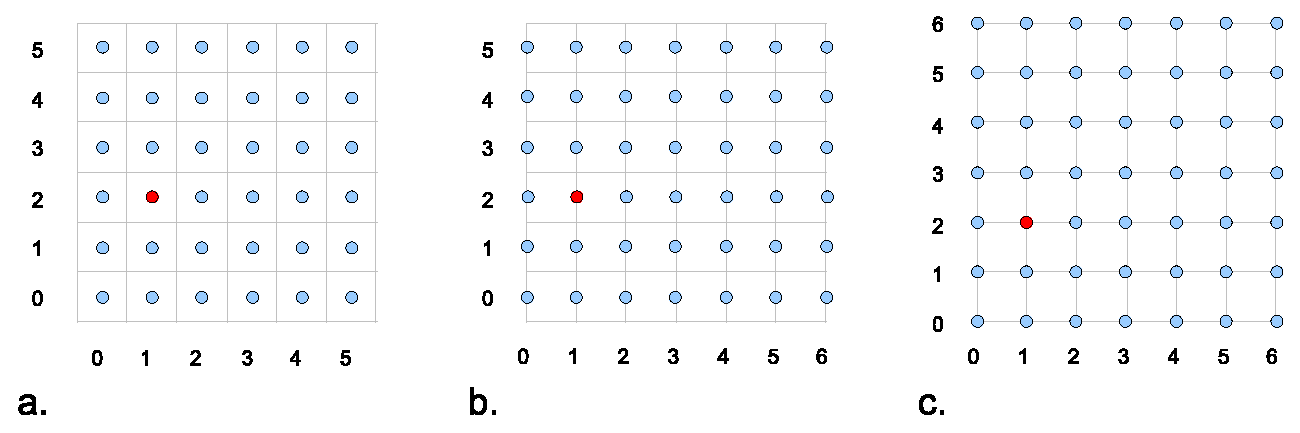
\includegraphics[width=6.5in]{\archfigpath/data_loc2}
\caption[Data-centerings on the grid]
  {\label{fig:dataloc} Some of the different data-centerings:
  (a) cell-centered, (b) nodal in the $x$-direction, and (c) nodal in
  both the $x$- and $y$-directions.  Note that for nodal data, the
  integer index corresponds to the lower boundary in that direction.
  In each of these centerings, the red point has the same indices:\ (1,2).
  Not shown is the case where data is nodal in the $y$-direction only.}
\end{figure}

\maestro's gridding is handled by the BoxLib library.  The underlying
idea in BoxLib is to allow for adaptive mesh refinement (AMR)---different
regions of the domain can have different spatial resolutions.  The
domain is broken into boxes.  At the coarsest (base) level of
refinement, the entire computational domain is covered, either by one
box or broken across many boxes.  Higher levels of refinement have
finer zones (typically $2\times$).  Only a portion of the domain may
be covered by the higher levels of refinement.  

\MarginPar{Nesting? ghost cells?}
For parallel computations, the boxes are spread across processors, in
a fashion designed to put roughly equal amounts of work on each
processor (load balancing).

On a grid, the data can be stored at cell-centers, on a face/edge, or
on the corners.  In BoxLib, data that is on an edge is termed `nodal'
in that direction (see Figure~\ref{fig:dataloc}).  Data that is on the
corners is nodal in all spatial directions.  In \maestro, the state
data (density, enthalpy, velocity, $\ldots$) is generally
cell-centered.  Fluxes are nodal in the direction they represent.
A few quantities are nodal in all directions (e.g.\ $\phi$ used in
the final velocity projection).

To simplify the description of the underlying AMR grid, BoxLib
provides a number of Fortran types.  We briefly summarize the major
data types below.


\subsection{\boxtype}

A \boxtype\ is simply a rectangular domain in space.  Note that boxes
do not hold the state data themselves.  A \boxtype\ has a {\tt lo} 
and {\tt hi} index in each coordinate direction that gives the
location of the lower-left and upper-right corner with respect to
a global index space.  

\begin{figure}[t]
\centering
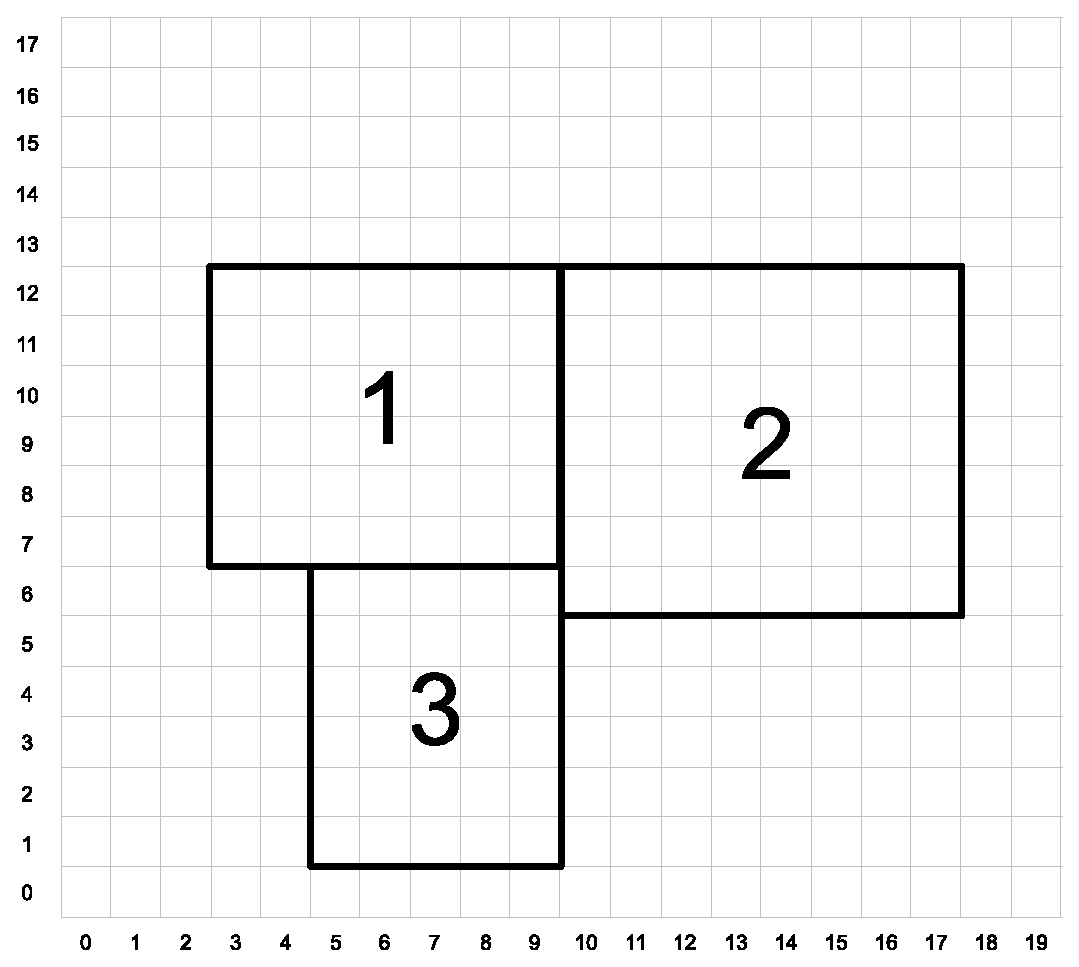
\includegraphics[width=4.0in]{\archfigpath/index_grid2}
\caption[Single-level grid structure]
{\label{fig:boxes} Three boxes that comprise a single level.  At this
  resolution, the domain is 20$\times$18 zones.  Note that the
  indexing in BoxLib starts with $0$.}
\end{figure}


The computational domain is divided into boxes.  The collection of
boxes with the same resolution comprise a level.
Figure~\ref{fig:boxes} shows three boxes in the same level of
refinement.  The position of the boxes is with respect to the global
index space at that level.  For example, box 1 in the figure has {\tt
  lo} = (3,7) and {\tt hi} = (9,12).  Note that the global indexing
is 0-based.

The global index space covers the entire domain at a given resolution.
For a simulation setup with {\tt n\_cellx = 32} and {\tt n\_celly =
  32}, the coarsest level (level 1) has $32 \times 32$ zones, and the
global index space will run from $0, \ldots, 31$ in each coordinate
direction.  Level 2 will have a global index space running from $0,
\ldots, 63$ in each coordinate direction (corresponding to $64 \times
64$ zones if fully refined), and level 3 will have a global index
space running from $0, \ldots, 127$ in each coordinate direction
(corresponding to $128\times 128$ zones if fully refined).


\subsubsection{Common Operations on a \boxtype}

A \boxtype\ declared as:
\begin{verbatim}
  type(box) :: mybox
\end{verbatim}
%
The upper and lower bounds of the box (in terms of the global
index space) are found via:
\begin{itemize}

\item {\tt lo = lwb(mybox)} returns an array, {\tt lo(dm)}, with
     the box lower bounds

\item {\tt hi = upb(mybox)} returns an array, {\tt hi(dm)}, with
     the box upper bounds

\end{itemize}




\subsection{\boxarray\ and \mlboxarray}

A \boxarray\ is an array of boxes.  A \mlboxarray\ is a collection of
\boxarray s at different levels of refinement.

\subsection{\layout\ and \mllayout}

A \layout\ is basically a \boxarray\ that knows information about other
boxes, or box ``connectivity.''  It contains additional information
that is used in filling ghost cells from other fine grids or from
coarser grids.  This information is stored as long as the layout
exists so that we don't have to recompute intersections every time we
do some operation with two \multifab s that have that layout, for
example.


\subsection{\fab}

A \fab\ is a ``Fortran Array Box''.  It contains the state data in a
multidimensional array and several \boxtype-types to describe where in
the global index-space it lives.  
Note that all state data is stored in a four-dimensional array,
{\tt (nx,ny,nz,nc)} in size, regardless of the dimensionality of the
problem.  Here {\tt nc} is the number of components, for instance
representing different fluid variables.  For 2D problems, {\tt nz=1}.

A \fab\ would represent the data for a single box in the domain.
In \maestro, we don't usually deal with \fab s alone, but rather
we deal with \multifab s, described next.

\subsection{\multifab}

A \multifab\ is a collection of \fab s at the same level of
refinement.  This is the primary data structure that \maestro\
routine operate on.  A multilevel simulation stores the 
data in an array of \multifab s, where the array index refers
to the refinement level.

\subsubsection{Working with \multifab s}

To build a \multifab, we need to provide a \layout, the number of
components to store in the \multifab\, and the number of ghostcells.  In
\maestro\, the hierarchy of grids will be described by a single
\mllayout.  A \multifab\ can be declared and built at any time in a
simulation using the \mllayout, thereby allocating space at every
grid location in the simulation.  The sequence to build a \multifab\
appears as
\begin{lstlisting}[language={[95]fortran},mathescape=false]
  type(multifab) :: mfab(nlevs)
  ...
  do n = 1, nlevs
     call multifab_build(mfab(n), mla%la(n), nc, ng)
  enddo
\end{lstlisting}
Here, {\tt nc} is the number of components and {\tt ng} is the number
of ghostcells.  The \multifab\ is built one level at a time, using the
\layout\ for that level taken from the \mllayout, {\tt mla}.

A common operation on a \multifab\ is to initialize it to $0$
everywhere.  This can be done (level-by-level) as
\begin{lstlisting}[language={[95]fortran},mathescape=false]
call setval(mfab(n), ZERO, all=.true.)
\end{lstlisting}
where {\tt ZERO} is the constant 0.0 from {\tt bl\_constants\_module}.

The procedure for accessing the data in each grid managed by the \multifab\
is shown in \S~\ref{sec:example}.  
Subroutines to add, multiply, or divide two \multifab s exist, as do
subroutines to copy from one \multifab\ to another---see {\tt boxlib/multifab.f90}
for the full list of routines that work with \multifab s.


When you are done working with a \multifab, its memory can be freed by
calling {\tt multifab\_destroy} on the \multifab.




\subsection{\bctower}

A \bctower\ holds the information about what boundary conditions are
in effect for each variable in a \maestro\ simulation.  \MarginPar{better description?}

\section{\maestro\ Data Organization}

The state of the star in \maestro\ is described by both a
multidimensional state and the 1D base state.  The full
multidimensional state is stored in \multifab s while the base state
is simply stored in Fortran arrays.  Here we describe the
major \maestro\ data-structures.




\subsection{`{\tt s}' \multifab s (fluid state)}

The fluid state (density, enthalpy, species, temperature, and tracer)
are stored together in a cell-centered multi-component \multifab,
typically named {\tt sold}, {\tt s1}, {\tt s2}, or {\tt snew}
(depending on which time-level it represents).  The enthalpy is stored
as $(\rho h)$, and the species are stored as partial-densities $(\rho
X_k)$.  The tracer component is not used at present time, but can
describe an arbitrary advected quantity.

Individual state variables should be indexed using the integer keys
provided by the {\tt variables} module (see \S
\ref{sec:variables_module}).  For example, the integer {\tt rho\_comp}
will always refer to the density component of the state.

Note: the pressure is not carried as part of the `{\tt s}' \multifab s.


\subsection{`{\tt u}' \multifab s (fluid velocity)}

The fluid velocity at time-levels $n$ and $n+1$ is stored in
a cell-centered multi-component \multifab, typically named
{\tt uold} or {\tt unew}.  Here the {\tt dm}
components correspond to each coordinate direction.

\subsection{{\tt umac} (the MAC velocity)}

In creating the advective fluxes, we need the time-centered velocity
through the faces of the zone---the $x$-velocity on the $x$-edges, the
$y$-velocity on the $y$-edges, etc.\ (see figure~\ref{fig:mac}).  This
type of velocity discretization is termed the MAC velocity (after the
``marker-and-cell'' method for free boundaries in incompressible
flows \cite{harlowwelch:1965}).



\begin{figure}[t]
\centering
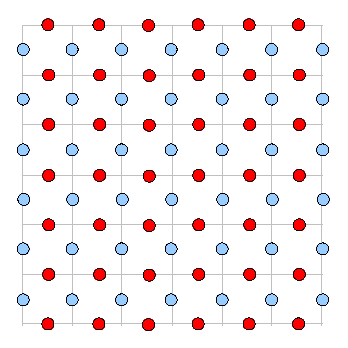
\includegraphics[width=2.5in]{\archfigpath/mac2}
\hspace{0.1in}
\begin{minipage}[b]{3.8in}
\caption[The MAC grid]
{\label{fig:mac} The MAC grid for the velocity.  
Here the $x$-velocity is on the $x$-edges (shown as the 
blue points) and the $y$-velocity is on the $y$-edges
(shown as the red points).
}\ \\
\end{minipage}
\end{figure}

The MAC velocities are allocated at each level of refinement, {\tt n},
by making a \multifab\ array where each of the {\tt dm} components is
nodal in its respective direction:
\begin{lstlisting}[language={[95]fortran},mathescape=false]
  type(multifab) :: umac(dm)

  do comp=1,dm
     call multifab_build_edge(umac(n,comp), mla%la(n),1,1,comp)
  enddo
\end{lstlisting}



\subsection{Base State Arrays}

The base state is defined by $\rho_0$, $p_0$, and $w_0$.  There is no
base state composition.  Other arrays are defined as needed, such as
$h_0$, the base state enthalpy.

The base state arrays are 2-dimensional, with the first dimension
giving the level in the AMR hierarchy and the second the radial index
into the base state.  For spherical geometries, the base state only
exists at a single level, so the first index will always be 1.  The
radial index is 0-based, to be consistent with the indexing for the
Cartesian state data.  For example, the base state density would be
dimensioned: {\tt rho0(nlevs,0:nr\_fine-1)}.  Here, {\tt nlevs} is the
number of levels of refinement and {\tt nr\_fine} is the number of
cells in the radial direction at the finest level of refinement.

For multilevel, plane-parallel geometry, all grids at the same height
will have the same resolution so that the full state data is always
aligned with the base state (see Figure~\ref{fig:base_state}).  Base
state data on coarse grids that are covered by fine grids is not
guaranteed to be valid.

For spherical problems, the base state resolution, $\Delta r$, is
generally picked to be finer than the Cartesian grid resolution,
$\Delta x$, i.e.\ $\Delta r < \Delta x$.  The ratio is controlled
by the parameter {\tt drdxfac}.



\section{\maestro\ Helper Modules}

A number of \maestro\ modules appear frequently throughout the source.
Below, we describe some of the more common functionality of the most
popular modules.

\subsection{\tt average}

The {\tt average} module provides a routine {\tt average} that takes
a multilevel \multifab\ array and averages the full Cartesian data
onto the 1D base state.

\subsection{{\tt eos\_module}}

The {\tt eos\_module} provides the interface to the equation of 
state to connect the state variables thermodynamically.  It 
gets the information about the fluid species from the {\tt network}
module (for example, the atomic number, $Z$, and atomic weight, $A$,
of the nuclei).

Presently there are 2 equations of state that work with \maestro:
\begin{itemize}
\item {\tt extern/EOS/helmeos/} represents a general stellar equation 
      of state, consisting of nuclei (as an ideal gas), radiation,
      and electrons (with arbitrary degeneracy and degree of relativity).
      This equation of state is that described in \cite{timmes_eos}.

\item {\tt extern/EOS/gamma\_law\_general} assumes an ideal gas with a mixed 
     composition and a constant ratio of specific heats, $\gamma$:
      \begin{equation}
      p = \rho e (\gamma - 1) = \frac{\rho k_B T}{\mu m_p} 
      \end{equation}
     where $k_B$ is Boltzmann's constant and $m_p$ is the mass of the
     proton.
     The mean molecular weight, $\mu$, is computed assuming 
     electrically neutral atoms:
     \begin{equation}
     \mu = \left ( \sum_k \frac{X_k}{A_k} \right )^{-1}
     \end{equation}
     An option in the source code itself exists for treating the
     species as fully-ionized, but there is no runtime-parameter to
     make this switch.
\end{itemize}

The {\tt eos\_module} declares for convenience the variables that need
appear in the {\tt eos} call argument list.  \maestro\ routines use
these module variables in the EOS call to avoid having to declare 
each quantity in each routine that calls the EOS.

The first argument to the {\tt eos} call is an integer key that
specifies which thermodynamic variables (in addition to the mass
fractions) are used as input.  EOS input options are listed 
in table~\ref{arch:table:eosinput}.

   \begin{table}[h]
   \caption{\label{arch:table:eosinput} EOS input flags}
   \begin{center}
   \begin{tabular}{lc}
   \hline
   key            & input quantities \\
   \hline
   {\tt eos\_input\_rt}       & $\rho$, $T$ \\
   {\tt eos\_input\_rh}       & $\rho$, $h$ \\
   {\tt eos\_input\_tp}       & $T$, $p$ \\
   {\tt eos\_input\_rp}       & $\rho$, $p$ \\
   {\tt eos\_input\_re}       & $\rho$, $e$ \\
   {\tt eos\_input\_ps}       & $p$, $s$ \\
   \hline
   \end{tabular}
   \end{center}
   \end{table}



\subsection{{\tt fill\_3d\_module}}

The {\tt fill\_3d\_module} provides routines that map from the 1D
base state to the full Cartesian 2- or 3D state.  Variations in the
routines allow for cell-centered or edge-centered data on either the
base state or full Cartesian state.

\subsection{{\tt geometry}}

\subsection{{\tt network}}

The {\tt network} module defines the number species advected by the
code ({\tt nspec}), their ordering, and gives their basic properties
(like atomic number, $Z$, and atomic mass, $A$).  All \maestro\ problems
require a {\tt network} module, even if there are no reactions
modeled.  Many different reaction modules (containing different sets
of isotopes) exist in {\tt extern/networks}.  The particular network
used by a problem is defined in the problem's {\tt GNUmakefile}.

To find the location of a particular species (for instance, ``carbon-12'')
in the allowed range of {\tt 1:nspec}, you do the following query:
\begin{lstlisting}[language={[95]fortran},mathescape=false]
  ic12 = network_species_index("carbon-12")
\end{lstlisting}
If the resulting index is {\tt -1}, then the requested species was not
found.

\subsection{{\tt probin\_module}}

\label{sec:probin}

{\tt probin\_module} provides access to the runtime parameters.
The runtime parameters appear simply as module variables.  To get the 
value of a parameter, one simply needs to `{\tt use probin\_module}'.
The preferred method is to add the `{\tt only}' clause to the
{\tt use} statement and explicitly list only those parameters that
are used in the routine.  Defining new runtime parameters is
described in \S~\ref{sec:def_runtime_param}.

\subsection{{\tt variables}}

\label{sec:variables_module}

The {\tt variables} module provides integer keys to index the state
multifabs and other arrays dealing with the scalar quantities.  The
most commonly used keys are are list in table~\ref{arch:table:variables}.

\begin{table}[h]
\caption{\label{arch:table:variables} Common {\tt variables} module keys}
\begin{center}
\begin{tabular}{ll}
\hline
{\tt rho\_comp}  & density \\
{\tt rhoh\_comp} & density $\times$ specific enthalpy, $(\rho h)$ \\
{\tt spec\_comp} & first species partial density, $(\rho X_1)$ \\
{\tt temp\_comp} & temperature \\
\hline
\end{tabular}
\end{center}
\end{table}

The species indices are contiguous in the state array, spanning {\tt
  spec\_comp:spec\_comp-1+nspec}.  To find a particular species, a
query can be made through the {\tt network} module, such as:
\begin{verbatim}
  ic12 = network_species_index("carbon-12")
\end{verbatim}
and then the \fab\ can be indexed using {\tt spec\_comp-1+ic12} to
get ``carbon-12''.
The {\tt variables} module also provides keys for the plotfile
variables and boundary condition types.

Other keys in the {\tt variables} modules are reserved for boundary
conditions ({\tt foextrap\_comp} and {\tt hoextap\_comp}), the
projection of the pressure ({\tt press\_comp}), or constructing
the plotfile.


\section{BoxLib Helper Modules}

There are a large number of modules in {\tt boxlib/} that provide
the core functionality for managing grids.  Here we describe
the most popular such modules.


\subsection{{\tt bl\_types}}

\subsection{{\tt bl\_constants}}

\subsection{{\tt parallel}}

\section{\label{sec:example} Example: Accessing State and MAC Data}

In \maestro, the state data is stored in a cell-centered multifab array
(the array index refers to the AMR level) and the MAC velocities are
stored in a 2D nodal multifab array (with indices referring to the AMR
level and the velocity component).  Here we demonstrate a typical way
to extract the state and MAC velocity data.

All \maestro\ routines are contained in a module, to allow for compile-time
argument checking.
\begin{lstlisting}[language={[95]fortran},mathescape=false]
module example_module

contains
\end{lstlisting}

The main interface to our routine is called {\tt example}---this will
take the \multifab s containing the data and then pass them to the
work routines, {\tt example\_2d} or {\tt example\_3d}, depending on
the dimensionality.  
\begin{lstlisting}[language={[95]fortran},mathescape=false]
  subroutine example(mla,s,umac,dx,dt)

    use bl_types
    use multifab_module
    use ml_layout_module
    use variables, only: rho_comp
\end{lstlisting}

\noindent Here, the {\tt bl\_types} and {\tt multifab\_module} modules
bring in the basic BoxLib data types. Specifically, here, {\tt
  bl\_types} defines {\tt dp\_t} which is the {\tt kind} used for
declaring double precision data, and {\tt multifab\_module} defines
the \multifab\ data type.  The {\tt ml\_layout\_module} defines the
datatype for a \mllayout---many routines will take an \mllayout
to allow us to fill ghostcells.  The {\tt variables} module is a \maestro\
module that provides integer keys for indexing the state arrays.  In
this case the integer {\tt rho\_comp} refers to the location in the
state array corresponding to density.

Next we declare the subroutine arguments:

\begin{lstlisting}[language={[95]fortran},mathescape=false]
    type(ml_layout), intent(in   ) :: mla
    type(multifab) , intent(inout) :: s(:)
    type(multifab) , intent(inout) :: umac(:,:)
    real(kind=dp_t), intent(in   ) :: dx(:,:),dt
\end{lstlisting}
Here, {\tt s(:)} is our \multifab\ array that holds the state data.
with the array index in {\tt s} refers to the AMR level.  The MAC 
velocities are held in the multifab {\tt umac}, with the array
indices referring to the AMR level and the component.


Local variable declarations come next:
\begin{lstlisting}[language={[95]fortran},mathescape=false]
    ! Local variables
    real(kind=dp_t), pointer :: sp(:,:,:,:)
    real(kind=dp_t), pointer :: ump(:,:,:,:), vmp(:,:,:,:), wmp(:,:,:,:)
    integer :: i,n,dm,nlevs,ng_sp,ng_um
    integer :: lo(mla%dim),hi(mla%dim)
\end{lstlisting}

\noindent Amongst the local variables we define here are a pointer,
{\tt sp}, that will point to a single \fab\ from the
\multifab\ {\tt s}, and a pointer for each component of the MAC
velocity, {\tt ump}, {\tt vmp}, and {\tt wmp} (for a 2D run,
we won't use {\tt wmp}).  We note that regardless of the dimensionality,
these pointers are 4-dimensional: 3 spatial + 1 component.

Next we get the dimensionality and number of levels
\begin{lstlisting}[language={[95]fortran},mathescape=false]
    dm = mla%dim
    nlevs = mla%nlevel
\end{lstlisting}


Each multifab can have their own number of ghostcells, so we get
these next:
\begin{lstlisting}[language={[95]fortran},mathescape=false]
    ng_sp = nghost(s(1))
    ng_um = nghost(umac(1,1))
\end{lstlisting}
By convention, all levels in a given multifab have the same number of
ghostcells, so we use level 1 in the {\tt nghost()} call.  We also use
the same number of ghostcells for each component of the velocity, so
we only need to consider the first component in the {\tt nghost()}
call.  The ghostcells will be needed to access the data stored in the
\fab s.

To access the data, we loop over all the levels, and all the boxes in
the given level.
\begin{lstlisting}[language={[95]fortran},mathescape=false]
    do n=1,nlevs
       do i = 1, nboxes(s(n))
\end{lstlisting}
{\tt nboxes(s(n))} is simply the number of boxes in level {\tt n}.
All data in all \multifab s will have the same box layout, so we only
need to query the number of boxes from one \multifab.

For a given \boxtype, we get the data and the bounds of the \boxtype.
\begin{lstlisting}[language={[95]fortran},mathescape=false]
          if ( multifab_remote(s(n), i) ) cycle
          sp  => dataptr(s(n), i)
          ump => dataptr(umac(n,1),i)
          vmp => dataptr(umac(n,2),i)
          lo =  lwb(get_box(s(n), i))
          hi =  upb(get_box(s(n), i))
\end{lstlisting}

\noindent For parallel runs, there is no guarantee that the particular
box is on the current processor.  The function {\tt multifab\_remote}
returns {\tt .true.} if the box is off-processor, in which case, we 
simply skip to the next box.

The actual data array is accessed through the {\tt dataptr} function,
which takes a \multifab\ (e.g.\ {\tt s(n)}) and the index of the
\boxtype\ ({\tt i}) we want.  We see that the $x$ MAC velocity for the
current box is stored in {\tt ump} and the $y$ MAC velocity is stored
in {\tt vmp}.  We don't get the $z$ velocity data here, since that
would not be available for a 2D run---we defer that until we test on
the dimensionality below.

Finally, the index bounds of the box (just the data, not the ghostcells) are 
stored in the {\tt dm}-dimensional arrays {\tt lo} and {\tt hi}.  These indices
refer to the current box, and hold for both the state, {\tt sp}, and the MAC
velocity, {\tt ump} and {\tt vmp}.  However, since the MAC velocity is nodal
in the component direction, the loops over the valid data will differ
slight (as we see below).

With the data extracted, we call a subroutine to operate on it.  We use
different subroutines for the different dimensionalities (and many times
have a separate routine for spherical geometries).
\begin{lstlisting}[language={[95]fortran},mathescape=false]
          select case (dm)
          case (2)
             call example_2d(sp(:,:,1,rho_comp),ng_sp, &
                             ump(:,:,1,1),vmp(:,:,1,1),ng_um, &
                             lo,hi,dx(n,:),dt)
          case (3)
             wmp => dataptr(umac(n,3),i)
             call example_3d(sp(:,:,:,rho_comp),ng_sp, &
                             ump(:,:,:,1),vmp(:,:,:,1),wmp(:,:,:,1),ng_um, &
                             lo,hi,dx(n,:),dt)
          end select
       enddo    ! end loop over boxes

    enddo    ! end loop over levels

  end subroutine example
\end{lstlisting}
\noindent We call either the function
{\tt example\_2d} for two-dimensional data or {\tt example\_3d}
for three-dimensional data.  Note that in the two-dimensional
case, we index the data as {\tt sp(:,:,1,rho\_comp)}.  Here a
`{\tt 1}' is used as the `z'-coordinate spatial index, since this
is a 2D problem, and the density component of the state is selected
(using the integer key {\tt rho\_comp}).  The 3D version accesses
the data as {\tt sp(:,:,:,rho\_comp)}---only the component regarding
the variable is needed here.  Notice that we also pass through
the number of ghostcells for each of the quantities.

This routine will be supplimented with {\tt example\_2d} and {\tt
example\_3d}, which actually operate on the data.  The form of 
the 2D function is:

\begin{lstlisting}[language={[95]fortran},mathescape=false]
  subroutine example_2d(density,ng_sp, &
                        umac,vmac,ng_um, &
                        lo,hi,dx,dt)

    use bl_constants_module
    use probin_module, only: prob_lo

    integer        , intent(in) :: lo(:),hi(:), ng_sp, ng_um
    real(kind=dp_t), intent(in) :: density(lo(1)-ng_sp:,lo(2)-ng_sp:)
    real(kind=dp_t), intent(in) ::    umac(lo(1)-ng_um:,lo(2)-ng_um:)
    real(kind=dp_t), intent(in) ::    vmac(lo(1)-ng_um:,lo(2)-ng_um:)

    real(kind=dp_t), intent(in) :: dx(:),dt

    integer         :: i, j
    real(kind=dp_t) :: x, y
    real(kind=dp_t) :: dens, u, v

    do j = lo(2), hi(2)
       y = prob_lo(2) + (dble(j) + HALF)*dx(2)

       do i = lo(1), hi(1)
          x = prob_lo(1) + (dble(i) + HALF)*dx(1)

          dens = density(i,j)

          ! compute cell-centered velocity
          u = HALF*(umac(i,j) + umac(i+1,j))
          v = HALF*(vmac(i,j) + vmac(i+1,j))

          ! operate on the data
          ! ...

       enddo
    enddo

  end subroutine example_2d

end module example_module
\end{lstlisting}

\noindent In this function, the bounds of the {\tt density} array take
into account the {\tt ng\_sp} ghostcells and the index space of the
current box.  Likewise, the MAC velocities refer to the {\tt ng\_um}
ghostcells.  The {\tt j} and {\tt i} loops loop over all the valid
zones.  Coordinate information is computed from {\tt dx} and {\tt
  prob\_lo} which is the physical lower bound of the domain.  {\tt
  bl\_constants\_module} declares useful double-precision constants,
like {\tt HALF} (0.5).  Here, we see how to access the density for
the current zone and compute the cell-centered velocities from the
MAC velocities.  By convection, for a nodal array, the indices refer 
to the {\em lower} interface in the nodal direction, so for {\tt umac},
{\tt umac(i,j)} and {\tt umac(i+1,j)} are the $x$ MAC velocities
on the lower and upper edge of the zone in the $x$-direction.

The three-dimensional case is similar, with the {\tt density} array
declared as 
\begin{lstlisting}[language={[95]fortran},mathescape=false]
  density(lo(1)-ng_sp:,lo(2)-ng_sp:,lo(3)-ng_sp:)
\end{lstlisting}
and an additional loop over the `z' coordinate (from {\tt lo(3)} to
{\tt hi(3)}).

In this example, we looped over the valid zones.  If we wished to loop
over the interfaces bounding the valid zones, in the $x$-direction,
we would loop as
\begin{lstlisting}[language={[95]fortran},mathescape=false]
  do j = lo(2), hi(2)
     do i = lo(1), hi(1)+1
        ! access umac(i,j)
     enddo
  enddo
\end{lstlisting}


\section{Filling Ghostcells}

Ghostcells are filled through a variety of different routines, depending
on the objective.

\begin{itemize}

\item {\tt multifab\_fill\_boundary} fills ghost cells for two
  adjacent grids at the same level, which als includes periodic domain
  boundary ghost cells.

\item {\tt multifab\_physbc} fills ghostcells at the physical boundaries.

\item {\tt multifab\_fill\_ghost\_cells} is used for multilevel
  problems, and fills ghostcells in the finer grid (level {\tt n}) by
  interpolating from data in the coarser grid (level {\tt n-1}).
  This function, by default, will also call {\tt multifab\_fill\_boundary}
  and {\tt multifab\_physbc} for both levels {\tt n} and {\tt n-1} (you 
  can override this behavior for speed optimization purposes).
  This call is usually preceded by a call to 
  {\tt ml\_cc\_restriction\_c} which sets the level {\tt n-1} data to be
  the average of the level {\tt n} data covering it.
   

\end{itemize}

\section{Boundary Conditions}


\section{Multigrid}

\maestro\ uses the multigrid solver to enforce the divergence constraint
both on the half-time edge-centered advective velocities (the ``MAC
projection'') and on the final cell-centered velocities (the ``HG
projection'').  For the MAC projection, since the velocity data is
edge-centered (the MAC grid), the projection is cell-centered.  For
the HG projection, since the velocity data is cell-centered, the
projection is node-centered.  \MarginPar{should draw a figure} The multigrid solver performs a number
of V-cycles until the residual drops by 10-12 orders-of-magnitude.
There are several options that affect how the multigrid solver
behaves, which we describe below.

\subsection{Special Bottom Solver}
We have a special bottom solver type that greatly speeds up large problems
and speeds up smaller problems to a lesser degree.
In fact, you should use this bottom solver whenever possible, because I
have yet to find a case that performs worse than our standard bottom solver.
What this special solver essentially does is take the data from the coarsest 
level of the original multigrid V-cycle and copy it onto a new grid structure 
with the same number of total cells in each direction, but with a fewer number of larger 
grids.  A new V-cycle begins from this point, 
so we are essentially coarsening this ``new'' problem.
Now, the coarsest level of the multigrid V-cycle in the ``new'' problem has 
fewer cells and fewer grids as compared to the original coarsest level.

To enable this solver, set {\tt hg\_bottom\_solver = 4} (for the nodal
projections) and/or {\tt mg\_bottom\_solver = 4} (for the cell-centered
projections) in your inputs file.

To understand how this bottom solver works, the first thing you need to know
is what the grid structure of the coarsest level of your multigrid V-cycle
looks like (we need to put a description of this in the section above).
Now, figure out the size of the box you would need if you
wanted it to fit all the data on the coarsest level.  Now, figure out what
the largest integer $n$ is so that you can evenly divide the length of this box
by $2^n$ in every coordinate direction.  If $n < 2$, the program will abort
since the grid structure is not suitable for this bottom solver.

Now the code will set up a ``new'' problem, using the data at the coarsest level
of the original problem as the initial data.  The grid structure for this new
problem has the same number of cells as the coarsest level of the original problem,
but the data is copied onto a grid structure where each grid has $2^n$ cells
on each side.  The new V-cycle continues down to the new coarsest level, in
which each grid has 2 cells on each side.  If you wish to impose a limit on
the maximum value that $n$ can have, you can do so by setting 
{\tt max\_mg\_bottom\_nlevs} equal to that value.

{\bf Example 1:} A 3D problem with $384^3$ cells divided into $32^3$ grids, i.e., 
there is a $12\times 12\times 12$ block of $32^3$ grids.  The coarsest level of the 
multigrid V-cycle contains $12\times 12\times 12$ grids that have $2^3$ cells, so the 
entire problem domain has $24^3$ cells.  We see that $n=3$, and create a new problem 
domain with a $3\times 3\times 3$ block of $8^3$ grids.  The coarsest level of the 
multigrid V-cycle for the ``new'' problem will be a $3\times 3\times 3$ block of 
$2^3$ grids.

{\bf Example 2:} A 2D problem with $96\times 384$ cells divided into $48^2$ grids, i.e., 
there is a $2\times 8$ block of $48^2$ grids.  The coarsest level of the multigrid 
V-cycle contains $2\times 8$ grids that have $3^2$ cells, so the entire problem 
domain has $6\times 24$ cells.  We see that $n=1$, so the program aborts since this grid
structure is not appropriate for the fancy bottom solver.


\section{Multilevel and Refinement Criteria}


\section{Particles}

\label{arch:sec:particles}

\maestro\ has support for Lagrangian particles that are passively
advected with the velocity field.  These are useful for diagnostics
and post-processing.  To use particles, particles must be seeded into
the domain by writing a problem-specific {\tt init\_particles.f90}
routine.  This routine is called at the start of the simulation.  The
{\tt init\_particles} routines add particles at specific locations by
calling the {\tt particle\_module}'s {\tt add} routine when a given
criteria is met by the fluid state.

When you run the code, particles are enabled by setting {\tt
  use\_particles = T}.  At the end of each timestep the locations of
all the particles are written out into a series of files called {\tt
  timestamp\_NN}, where {\tt NN} is the CPU number on which the
particle {\em currently} resides.  Particles are always kept on the
processor containing the state data corresponding to their present
location.  Several bits of associated data (density, temperature, and
mass fractions) are stored along with the particle ID and position.

Some simple python scripts allow for the plotting of the particle
positions.  See \S~\ref{analysis:sec:particles} for details.


